\documentclass{beamer}
\usepackage[utf8]{inputenc}

\usetheme{Madrid}
\usecolortheme{default}
\usepackage{amsmath}
\usepackage{amssymb,amsfonts,amsthm}
\usepackage{txfonts}
\usepackage{tkz-euclide}
\usepackage{listings}
\usepackage{adjustbox}
\usepackage{array}
\usepackage{tabularx}
\usepackage{gvv}
\usepackage{lmodern}
\usepackage{circuitikz}
\usepackage{tikz}
\usepackage{graphicx}

\setbeamertemplate{page number in head/foot}[totalframenumber]

\usepackage{tcolorbox}
\tcbuselibrary{minted,breakable,xparse,skins}



\definecolor{bg}{gray}{0.95}
\DeclareTCBListing{mintedbox}{O{}m!O{}}{%
  breakable=true,
  listing engine=minted,
  listing only,
  minted language=#2,
  minted style=default,
  minted options={%
    linenos,
    gobble=0,
    breaklines=true,
    breakafter=,,
    fontsize=\small,
    numbersep=8pt,
    #1},
  boxsep=0pt,
  left skip=0pt,
  right skip=0pt,
  left=25pt,
  right=0pt,
  top=3pt,
  bottom=3pt,
  arc=5pt,
  leftrule=0pt,
  rightrule=0pt,
  bottomrule=2pt,
  toprule=2pt,
  colback=bg,
  colframe=orange!70,
  enhanced,
  overlay={%
    \begin{tcbclipinterior}
    \fill[orange!20!white] (frame.south west) rectangle ([xshift=20pt]frame.north west);
    \end{tcbclipinterior}},
  #3,
}
\lstset{
    language=C,
    basicstyle=\ttfamily\small,
    keywordstyle=\color{blue},
    stringstyle=\color{orange},
    commentstyle=\color{green!60!black},
    numbers=left,
    numberstyle=\tiny\color{gray},
    breaklines=true,
    showstringspaces=false,
}
\title{1.9.14}
\date{27th August, 2025}
\author{Vishwambhar - EE25BTECH11025}

\begin{document}

\frame{\titlepage}
\begin{frame}{Question}
If $\vec{P}=\brak{2,2}$, $\vec{Q}=\brak{-4,-4}$, and $\vec{R}=\brak{5,-8}$ are the vertices of a triangle $\Delta PQR$, then find the length of the median through $\vec{R}$.\\
\end{frame}

\begin{frame}{allowframebreaks}
\frametitle{Midpoint of $\vec{Q}-\vec{P}$}
Given position vectors of the points are:
\begin{align}
    \vec{P}=\myvec{2\\2},
    \vec{Q}=\myvec{-4\\-4},
    \vec{R}=\myvec{5\\-8}
\end{align}
Let the midpoint of vector $\vec{Q}-\vec{P}$ be $\vec{M}$:
\begin{align}
    \vec{M}=\frac{1}{2}\vec{P}+\frac{1}{2}\vec{Q}\\
    \vec{M}=\myvec{1\\1}+\myvec{-2\\-2}\\
    \vec{M}=\myvec{-1\\-1}
\end{align}
\end{frame}

\begin{frame}[fragile]
\frametitle{Length of Median}
\begin{align}
    \vec{M}-\vec{R}=\myvec{-1\\-1}-\myvec{5\\-8}\\
    \vec{M}-\vec{R}=\myvec{-6\\7}
\end{align}

The length of the median:
\begin{align}
    ||\vec{M}-\vec{R}||=\sqrt{\brak{-6}^2+\brak{7}^2}\\
    ||\vec{M}-\vec{R}||=\sqrt{85}\approx9.219
\end{align}

Thus the length of the median of the triangle through $\vec{R}$ is $\sqrt{85}\approx9.219$.
\end{frame}

\begin{frame}[fragile]
    \frametitle{C Code}
    \begin{lstlisting}
#include <stdio.h>
#include <math.h>
void make_data(double *points) {
    double Px = 2; double Py = 2;
    double Qx = -4; double Qy = -4;
    double Rx = 5; double Ry = -8;
    double Mx = (Px + Qx)/2; double My = (Py + Qy)/2;
    double value = sqrt(((Mx - Rx)*(Mx - Rx))+((My - Ry)*(My - Ry)));
    points[0] = Px;points[1] = Py;
    points[2] = Qx;points[3] = Qy;
    points[4] = Rx;points[5] = Ry;
    points[6] = Mx;points[7] = My;
    points[8] = value;
}
    \end{lstlisting}
\end{frame}

\begin{frame}[fragile]
    \frametitle{Python Code 1}
    \begin{lstlisting}
import ctypes as ct
import numpy as np

def get_data():
    lib = ct.CDLL("./problem.so")

    value = ct.c_double*9

    lib.make_data.argtypes = [ct.POINTER(ct.c_double)]

    points = value()

    lib.make_data(points)
    \end{lstlisting}
\end{frame}

\begin{frame}[fragile]
    \frametitle{Python Code 1}
    \begin{lstlisting}
    Px = points[0] 
    Py = points[1]
    Qx = points[2]
    Qy = points[3]
    Rx = points[4]
    Ry = points[5]
    Mx = points[6]
    My = points[7]
    values = points[8]
    return Px, Py, Qx, Qy, Rx, Ry, Mx, My, values
    \end{lstlisting}
\end{frame}

\begin{frame}[fragile]
    \frametitle{Python Code 2}
    \begin{lstlisting}
import numpy as np
import matplotlib.pyplot as plt
from call import get_data

Px, Py, Qx, Qy, Rx, Ry, Mx, My, values = get_data()

a = ([Px, Qx, Rx, Mx, Px, Rx])
b = ([Py, Qy, Ry, My, Py, Ry])

plt.plot(a, b, color = 'black')

plt.text(Px, Py, 'P', fontsize=12, color = 'red')
plt.text(-4.4, -3.9, 'Q', fontsize=12, color = 'red')
    \end{lstlisting}
\end{frame}

\begin{frame}[fragile]
    \frametitle{Python Code}
    \begin{lstlisting}
plt.text(Rx, Ry, 'R', fontsize=12, color = 'red')
plt.text(-1.1, -0.8, 'M', fontsize=12, color = 'red')

plt.xlabel('X-axis')
plt.ylabel('Y-axis')
plt.axis('equal')
plt.grid(True)
plt.savefig('../figs/plot.png')
plt.show()

    \end{lstlisting}
\end{frame}

\begin{frame}{Plot}
    \begin{figure}
        \centering
        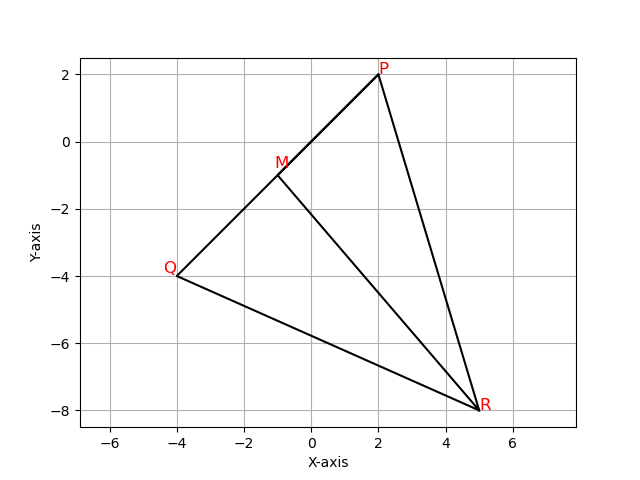
\includegraphics[width=0.5\columnwidth]{../figs/plot.png}
        \caption{Plot of triangle PQR along with median}
        \label{fig:fig}
    \end{figure}
\end{frame}




\end{document}
